\documentclass[10pt,a4paper]{report}
\setcounter{tocdepth}{5}
\setcounter{secnumdepth}{5}
\usepackage{graphicx}
%\usepackage{float}
\usepackage{subfig}
%\usepackage{graphicx}
\usepackage{subcaption}
\usepackage{indentfirst}
\usepackage[export]{adjustbox}
\usepackage{hyperref}
\usepackage{color,soul}
%\usepackage{amsmath}
%\usepackage{algorithm}
%\usepackage{algpseudocode}
%\usepackage[ruled,linesnumbered]{algorithm2e}

\usepackage{blindtext}
%\usepackage{booktabs}
\usepackage{caption}
\usepackage{tikz}
\usepackage[english]{babel}
\usepackage[sort,comma,numbers]{natbib}
\usepackage[final]{pdfpages}
\usepackage{setspace}
\usepackage{titlesec}
\usepackage{ragged2e}
\usepackage{listings}%
%\usepackage{bm}
\usepackage{multirow}

%\usepackage{graphicx}
%\usepackage{multirow}
\usepackage{amsmath}
\usepackage{amssymb}

\usepackage{booktabs}
\usepackage{float}

\usepackage{algpseudocode}
\usepackage[ruled,linesnumbered]{algorithm2e}


\usepackage{enumitem}

\usepackage{pifont}% http://ctan.org/pkg/pifont
\newcommand{\cmark}{\ding{51}}
\newcommand{\xmark}{\ding{55}}

\usepackage{hhline}

\usepackage{bm}

\usepackage{diagbox}
%\usepackage{natbib}
\usepackage{titlesec}



\usepackage{graphicx}
\usepackage{url}


\definecolor{lightblue}{rgb}{.80,.85,1}
\sethlcolor{lightblue}





% Customize chapter heading
\titleformat{\chapter}[display]
  {\normalfont\huge\bfseries} % Format for chapter title
  {\chaptername\ \thechapter} % Label format (e.g., Chapter 1)
  {20pt} % Space between label and title
  {\Huge} % Chapter title format
  [\vspace{2ex}\titlerule] % Format for the title separator (line)

% Customize section heading
\titleformat{\section}
  {\normalfont\Large\bfseries} % Format for section title
  {\thesection} % Label format (e.g., 1.1)
  {1em} % Space between label and title
  {} % Before code
  [] % After code

% Adjust spacing before and after section headings
\titlespacing{\section}{0pt}{0.85cm}{0.85cm}
\titlespacing{\subsection}{0pt}{0.75cm}{0.75cm}
\titlespacing{\subsubsection}{0pt}{0.5cm}{0.5cm}

% Customize Acknowledgements, Declaration, and Contents headings without the line and less space
\titleformat{name=\chapter,numberless}[display]
  {\normalfont\huge\bfseries}
  {}
  {20pt}
  {\Huge}
  [\vspace{1ex}]  % Adjust this value to reduce space

% Specific customization for Declaration
\newcommand{\declarationtitleformat}{%
  \titleformat{name=\chapter,numberless}[display]
    {\normalfont\huge\bfseries}
    {}
    {10pt} % Adjust this value to reduce space
    {\Huge}
    [] % No line after title
}


\begin{document}


\newpage
\thispagestyle{empty}
\pagenumbering{gobble}
%%%%%%%%%%%%%%%%%%%%%%%%%%%%%%%%%%Title Page%%%%%%%%%%%%%%%%%%%%%%%%%%%%
\begin{titlepage}
	\begin{center}
		{\Large\textbf{Technical Report}}\\ \large{\textbf{Upgradation from UGC-NET JRF to SRF\\under UGC (NFOBC) scheme}}
		\vspace{1cm}\\
            \textbf{Harinath Kuruva}\\
            \textbf{Reg. No. 21MCPC07}\\
		\vspace{1cm}
		\large Supervisors\\ 
		\large \textbf{Prof. K. Swarupa Rani}\\
            \large \textbf{Prof. Salman Abdul Moiz}\\
		\vspace{1cm}
            \large DRC Members\\ 
		\large \textbf{Dr. K. Anjeneya Swami}\\
            \large \textbf{Prof. P.S.V.S Sai Prasad}\\
		\vspace{1cm}
        
\includegraphics[scale=1.5]{images/UoH.png} \\
        \vspace{0.5cm}
        \large School of Computer and Information Sciences \\
		\textbf{University of Hyderabad} \\
		Gachibowli, Hyderabad - 500 046 \\
		Telangana, India \\
		\vspace{0.5cm}
		\textbf{\today}
	\end{center}
\end{titlepage}





% Reset title format for subsequent sections
\titleformat{name=\chapter,numberless}[display]
  {\normalfont\huge\bfseries}
  {}
  {20pt}
  {\Huge}
  [\vspace{1ex}]
  



\newpage
\pagenumbering{arabic}
\titleformat{\chapter}[display]
  {\normalfont\bfseries}{}{0pt}{\Huge} % Format for chapter title
  %{\chaptername\ \thechapter} % Label format (e.g., Chapter 1)
  %{20pt} % Space between label and title
  %{\Huge} % Chapter title format
  %[\vspace{2ex}\titlerule] % Format for the title separator (line)




\Large{\textbf{Status of the work from $25^{th}$ October 2021 till date}}
\begin{enumerate}
    \item \large{\textbf{Completed Course Work}}
    \begin{itemize}
        \item Research Methods in Computer Science - Core Course 
        \item Data Structures And Programming Lab - Core Course
        \item Algorithms - Core Course
        \item Research Publications and Ethics - Core Course
        \item Machine Learning - Elective Course
        \item Social Network Analysis - Audit Course
    \end{itemize}
    \item \large{\textbf{Survey of Visualization Recommendation and NLDR approaches}}
    \begin{itemize}
        \item Extensive survey on Visualization recommendation \sloppy{approaches} can be categorized into visualization selection, technique, and recommendation.
        \item Extension survey on nonlinear dimensionality reduction approaches which can visualize the high-dimensional data.
    \end{itemize}
    
    \item \large{\textbf{Contribution 1:}}\\
    \justifying{Kuruva, H., Swarupa Rani, K., Moiz, S.A. (2023). \textbf{Visualization Recommendation for Incremental Data Based on Intent.} In: Morusupalli, R., Dandibhotla, T.S., Atluri, V.V., Windridge, D., Lingras, P., Komati, V.R. (eds) Multi-disciplinary Trends in Artificial Intelligence. MIWAI 2023. Lecture Notes in Computer Science, vol 14078. Springer, Cham. \url{https : //doi.org /10.1007/978−3−031−36402−0 26}}
    
    \item \large{\textbf{Contribution 2:}}\\
    Proposed $HM\_QCv$: A Computationally Efficient Hybrid Model for Enhancing Quality Clusters in Visualization - \textbf{Communicated to Big Data Research Journal (Special Issue) on $21^{st}$ Jan 2025.}
    \item \large{\textbf{Contribution 3:}}\\
    Proposing a framework for Incremental Visualization Recommendation using Feature Selection.
\end{enumerate}


The contributions are discussed in the Sections 3, 4 and 5.
\chapter{Introduction}

There is a beautiful saying, ``a picture is worth a thousand words'', which gives the essence of the importance of visualization. Humans are able to visualize the world, so it is easier to process data in a visual context. Data Visualization is a pictorial representation that transforms data into visual elements. Nowadays, users are required to analyze the data with the help of visualization. Visualization can be a powerful tool for communication, analysis, and decision-making. Visualization has many real-world applications in various fields like Business and Finance, Healthcare, Sports, Education, Science and Engineering. Data visualization plays a vital role in business and healthcare, enabling decision-makers to quickly comprehend complex information and make informed decisions. In Business and Finance, it can analyze financial data, such as stock prices, sales figures, and customer behavior, to identify trends and make better business decisions. Data visualization transforms data into visual representations such as charts, graphs, and maps, making the data easier to process, analyze, and interpret. Maps and graphs are frequently used for a better understanding of concepts rather than having long textual paragraphs. On one hand usage of maps and charts in daily life is increasing and it is an example of visualization. On the other hand data has been increasing rapidly over the internet and there is a need to represent and also provide insights to the data by applying visualization techniques. Therefore, data visualization plays a vital role in having a brief insight into the information.

A visualization is recommended to the user by satisfying their requirements for a particular dataset. There have been many approaches like rule-based, machine learning approaches, knowledge graph embedding \sloppy{approaches} for recommending the visualization for the dataset. These approaches recommend visualization based on the rules, training a machine learning model by extracting features of data and by constructing knowledge graph from the data respectively. As per our study there was an approach of Maruta et al. \cite{maruta2021intent} works related to the visualization recommendation based on intent from the user. Intent is an english sentence that says about the requirement from the user. Using the intent for visualization recommendation makes the task easy to analyze and to provide accurate results desired by the user. 

High dimensional data visualization refers to the techniques used to represent and display data that exists in more than three dimensions. The challenge in high-dimensional data visualization is the curse of dimensionality. As the number of dimensions in a dataset increases, the amount of data required to adequately cover the space grows exponentially. This means that high-dimensional datasets may be sparse, making it difficult to draw meaningful insights from the data. To address this challenge, the intent based incremental approach is used.

Incremental visualization is a technique used in data visualization where data is updated dynamically in real-time. With the context of volume and velocity of big data which is being added to the existing data, it has been very difficult to provide visualization recommendation for incremental data. This challenge is addressed by our proposed approach (IVR\_I) which can handle challenges posed by volume and velocity. Our approach will recommend visualization to the incremental data by executing the visualization recommendation algorithm only on the incremental data, not from scratch (updated data). Hence, our proposed methodology is taking less time.

\section{Significant Contributions of IVR\_I} 
\begin{itemize}
    \item Developed and proposed IVR algorithm.
    \begin{itemize}
        \item Let p be our proposed algorithm, z is visualization recommendation, x be the existing data, hy is horizontal increment and vy is vertical increment.
        \begin{itemize}
            \item If \( p(x) \rightarrow z\) and \(p(hy) \rightarrow z\) then we can say \(p(x+(hy)) \rightarrow z\)
            \item If \( p(x) \rightarrow z\) and \(p(vy) \rightarrow z\) then we can say \(p(x+(vy)) \rightarrow z\)
        \end{itemize}
        \item Visualization recommendation for horizontal and vertical increments of data.
    \end{itemize}
\end{itemize}

Several data visualization techniques \cite{belkin2003laplacian,sammon1969nonlinear,Hinton2002,tsne,umap_reference,roweis2000nonlinear} transform high-dimensional data into lower dimensions, making it easier to interpret and analyze. Dimensionality reduction techniques can be broadly categorized into Linear and Non-Linear approaches. The Linear approach will reduce the dimensions by linearly mapping the features of the data. Linear approaches, such as PCA \cite{jolliffe2002principal}, are unsuitable for high-dimensional data, as they can only capture linear relationships within the data. The Non-Linear approach is suitable for visualizing data based on essential characteristics by maintaining (i) the global structure and (ii) the local structure of the data. These characteristics help to provide deeper insights and a more accurate representation of complex patterns.

Most of the Non-Linear approaches \cite{tsne} \cite{umap_reference} in the literature primarily focused on retaining partial characteristics by preserving either the local structure or the global structure of the data. t-SNE \cite{tsne} approach visualizes the data by calculating the similarities of high-dimensional data and mapping them with those of low-dimensional data using a loss function. This approach has a drawback where much computation is involved while calculating the similarities of the data points.  UMAP \cite{umap_reference} generates a high-dimensional graph representation of the data, then constructs a similar low-dimensional graph, minimizing cross-entropy to preserve the original information in the reduced dimensional space.  This approach is more computationally efficient and robust in handling outliers than t-SNE \cite{tsne}. However, it may struggle to handle small datasets, resulting in overfitting or noisy visualizations.

Visualizing the clusters is crucial in marketing and medicine to extract insights, identify patterns,  group customers based on behavior, and make better decisions. t-SNE \cite{tsne} preserves local structures but does not guarantee the preservation of global structures. UMAP \cite{umap_reference} focuses more on preserving global structures but can't guarantee the preservation of local structures. UMAP \cite{umap_reference} is more computationally efficient than t-SNE \cite{tsne}. 

LAPtSNE \cite{sun2023laplacian}, leverages eigenvalues from the Laplacian graph matrix to form desired visual clusters in the reduced dimensional space by preserving both local and global structures. However, LAPtSNE \cite{sun2023laplacian} can preserve local and global structures but inherits computational challenges due to its adaptation of the t-SNE \cite{tsne} methodology to preserve the local structure. 



Given the limitations of existing techniques and the increasing demand for real-world applications, there is a need for a new approach that can handle all types of characteristics involved with each of these methods and should be computationally efficient. Hence, we propose a novel approach, \textbf{\underline{H}}ybrid \textbf{\underline{M}}odel for \textbf{\underline{Q}}uality \textbf{\underline{C}}lusters in \underline{$\bm{v}$}isualization ($HM\_QCv$), which is a computationally efficient and comprehensive solution for high-dimensional data, capable of forming quality visual clusters by preserving local and global structures and robustly handling outliers. 






\section{Significant Contributions of \texorpdfstring{$HM\_QCv$}{HM\_QCv}}
%Significant contributions are as follows:
\begin{itemize}
    \item The $HM\_QCv$ algorithm stands out for its computational efficiency, constructing a graph by minimizing the cross-entropy between high-dimensional and low-dimensional representations. It effectively captures high-dimensional data while being robust to outliers.
    \item The $HM\_QCv$ algorithm, a key contribution of this research work, efficiently generates cluster-effective visualizations by leveraging the existing methods to enhance quality clusters in high-dimensional data.
    \item The proposed approach preserves both the local and global structures in high-dimensional data.
\end{itemize}















\chapter{Related Work}
Dimensional stacking is a visualization technique that allows for the simultaneous display of multiple dimensions or categories of data within a single plot. It involves stacking multiple two-dimensional plots on top of each other, with each plot representing a different category or dimension of the data. While dimensional stacking can be a useful technique for visualizing multiple dimensions of data, there are also other techniques available for multidimensional visualization. There will be no clarity in this technique as all dimensions are plotted instead the visualization techniques like bivaraite and univariate techniques are used in our methodology.

\section{Visualization Recommendation Approaches}
Visualization recommendation approaches can be divided into rule based, machine learning and  knowledge graph approaches. Rule based visualization recommendation approaches will be constructing the rules depending on the type of the data in the dataset and with the help of experts intervention. Examples of rule based approaches include APT \cite{mackinlay1986automating}, Show Me\cite{mackinlay2007show} SAGE \cite{roth1994interactive} and Voyager2 \cite{wongsuphasawat2017voyager}. The disadvantage is that it requires a lot of human effort for constructing the rules.  Contrasting to rule based approaches, machine learning based approaches will be extracting the features from the dataset and those extracted features are given to machine learning models for predicting the visualization of a particular dataset.  Qian et al., \cite{qian2020ml} and Hu et al., \cite{hu2019vizml} are examples of machine learning based approaches. These approaches use neural networks which is a black box where we are unable to know why the particular visualization is recommended. Knowledge graph based approaches such as KG4Vis \cite{li2021kg4vis} will construct the knowledge graph from the visualization corpus and use the graph to recommend the visualization. Constructing the knowledge graph is the main hindrance in this approach which is mainly dependent on a large corpus of the data. There are several other approaches that are related to the visualization recommendation in different contexts which are discussed below.

Lee et.al., \cite{lee2021lux} approach extracts information from the data frames and recommends the visualization. Epperson et.al., \cite{epperson2022leveraging} recommend the visualization based on the history of a user’s data analysis. Ojo et.al., \cite{ojo2022visgnn} recommend personalized visualization by constructing Graph Neural Network from the large corpus of the data. Harris et.al., \cite{harris2021insight} recommend visualization by utilizing relevant insights in the data. Gao et.al., \cite{gao2021vizgrank} obtained all possible visualizations for the given dataset, constructed a graph by modeling the relations between all visualizations, and finally recommended the high score visualization. Kelleher et.al., \cite{kelleher2021introductory} provided the visualization recommendation for scientific datasets in the context of big data. 
The above discussed approaches deal with different dataset for visualization recommendation. There exists an approach Maruta et al. \cite{maruta2021intent}  which is based on two input parameters such as intent and dataset used for visualization recommendation. Intent refers to information that actually the user desires to visualize from the dataset.



Apart from visualization recommendation approaches discussed earlier there is a need to know about incremental visualization in order to solve the problem of visualization recommendation for incremental data. Incremental visualization \cite{schulz2015enhanced} is a technique used in data visualization where data is updated dynamically in real-time. There is no efficient strategy in the literature to address incremental visualization recommendation. In this paper we proposed the methodology to solve this problem without rendering an entire chart or graph for every time stamp which can save significant processing time and improves the user experience. We extended the works of Maruta et al. \cite{maruta2021intent} which recommends the visualization based on two input parameters such as the intent and dataset provided by the user for incremental data.

\section{Exploring basic NLDR techniques}
Non-Linear Dimensionality Reduction (NLDR) approaches are indispensable for visualizing high-dimensional data, especially when linear methods are inadequate for capturing intricate data
structures. Techniques such as t-SNE \cite{tsne}, UMAP \cite{umap_reference}, and Laplacian-based methods \cite{belkin2001laplacian} \cite{sun2023laplacian} play a crucial role in preserving local and global structures by projecting data into lower dimensional
spaces while retaining meaningful patterns. These methods are particularly effective in
uncovering non-linear relationships, making them invaluable for exploring and understanding
complex datasets, especially in fields like healthcare and marketing.


An approach like Sammon Mapping \cite{henderson1997sammon} minimizes the difference between pairwise distances in the high-dimensional data and their corresponding distances in the low-dimensional representation. Curvilinear Component Analysis \cite{demartines1995cca} identifies a low-dimensional data representation that maximizes the correlation between the actual and low-dimensional data points. Isomap \cite{tenenbaum2000global} improves traditional MDS \cite{hout2013multidimensional} by including geodesic distances, making it ideal for nonlinear manifolds. SNE \cite{hinton2002stochastic} maintains the pairwise similarities between data points by applying probability distributions while transforming high-dimensional data into low-dimensional data and capturing local structures.

\section{From Neighbourhood to Topologies: Embedding High-Dimensional Data}

SNE \cite{hinton2002stochastic} minimizes the Kullback-Leibler (KL) divergence between the probability distributions in low and high-dimensional spaces. t-SNE \cite{tsne} effectively maps high-dimensional data to a low-dimensional space while preserving pairwise similarities between data points, unlike its predecessor, SNE \cite{hinton2002stochastic}, which relies on asymmetric conditional probabilities. High-dimensional similarities are modeled using Gaussian distributions, whereas low-dimensional similarities leverage a student-t distribution with one degree of freedom, providing heavy tails to capture the influence of outliers. t-SNE \cite{tsne} introduces symmetric joint probabilities, resulting in a symmetric and more stable cost function. Through gradient descent optimization, t-SNE \cite{tsne} overcomes SNE’s limitations by improving complex data handling for visualization and analysis. However, the authors claim that it preserves global structure to some extent and is computationally intensive.


McInnes et al. \cite{umap_reference} discovered UMAP, the NLDR technique, which creates a high-dimensional graph, and then a similar graph in lower dimensions is determined. UMAP relies on strong theoretical principles of riemannian manifolds \cite{lin2008riemannian} and preservation of topological structure. UMAP operates through two key phases: (1) the construction of a high-dimensional graph and (2) the optimization of low-dimensional embedding. 


In the first phase, a graph is constructed by identifying the k-nearest neighbours of each data point $x_i$ in high-dimensional space using pairwise distances. The high-dimensional probabilities are calculated to represent the fuzzy membership strengths between data points. A weighted k-nearest neighbour graph is then constructed. To symmetrize the adjacency matrix, UMAP applies a transformation, combining the matrix with its transpose.


In the second phase, the low-dimensional space is initialized randomly, and its probabilities are computed for each pair of points based on their distances, with hyperparameters \textit{`a'} (scaling factor) and \textit{`b'} (decay rate). The final low-dimensional embedding is optimized by minimizing the cross-entropy between the high-dimensional and low-dimensional representations, ensuring the structural similarities are preserved. UMAP \cite{umap_reference} uses stochastic gradient descent to iteratively refine the positions of the points, effectively embedding the high-dimensional data in a low-dimensional space while maintaining global structures, and these authors also claimed that it does not guarantee the local structure.


UMAP \cite{umap_reference} outperforms t-SNE \cite{tsne} in preserving global structures and is scalable for large datasets. This approach provides good visualizations and is computationally less expensive than t-SNE, making it suitable for real-time datasets.


\section{Exploring Laplacian Eigenmaps and LAPtSNE}

Laplacian Eigenmaps \cite{belkin2001laplacian}, a spectral graph-based technique, preserves the local structure of the data. It achieves this by creating a graph with nodes representing data points and edges reflecting their neighbourhood associations. The approach then computes the Laplacian matrix for the created graph and, based on these values, further calculates eigenvalues to determine a lower-dimensional data embedding. This embedding minimizes the cost function by ensuring that the closeness between data points in the high-dimensional space remains the same in the low-dimensional space. Laplacian Eigenmaps are highly effective in capturing the multidimensional structure of data and particularly helpful for clustering the data in visualization space. 

Sun et al., \cite{sun2023laplacian} developed the LAPtSNE approach that uses the base t-SNE algorithm. This approach preserves both local and global structures in high-dimensional space, resulting in compact cluster visualization in low-dimensional embedding. The process begins by applying t-SNE to compute pairwise affinities in the high-dimensional data. Further, the graph laplacian matrix is calculated based on the affinity matrix of t-SNE. The \textit{`d'} number of the smallest eigenvectors of the Laplacian matrix is used to initialize the low-dimensional embedding. 

In each iteration of LAPtSNE, low-dimensional probabilities are computed using a student-t distribution, similar to the standard t-SNE process. The LAPtSNE algorithm operates in an iterative manner, continually refining the low-dimensional embedding. The gradient of the KL divergence between high and low-dimensional affinities is estimated and regularized. The low-dimensional embeddings are updated with the calculated values to minimize the model’s KL divergence and the regularization factor to preserve neighbourhood relations. This iterative process is crucial in refining the low-dimensional embedding while preserving the global structure and cluster integrity.


An approach like t-SNE \cite{tsne} preserves the local structure but claims to retain the global structure partially to some extent. UMAP \cite{umap_reference} focuses more on preserving the global structure but does not guarantee the local structure. LAPtSNE \cite{sun2023laplacian} can preserve both local and global structures with cluster visualization quality, but it is computationally intensive for high-dimensional datasets.  Therefore, there is a need to discover a computationally efficient NLDR approach that can preserve both local and global structures and produce high-quality cluster visualizations for high-dimensional data.

\chapter{\Large Visualization Recommendation for Incremental Data based on Intent (IVR\_I)}


Our proposed approach is discussed to handle the incremental data that has been generated over time in the real world. Nowadays, data is growing tremendously in an incremental fashion. The data can be added in terms of volume in big data in a dynamic environment horizontally (instances are added) or/and vertically (new dimensions are added). It is quite challenging to provide the visualization recommendation in this situation and the problem remained unaddressed. There are many approaches for recommending the visualization for entire data (existing and incremental data) but they are time consuming and very expensive because considering the entire data from the scratch and repeating this procedure. To address this issue, our approach recommends the visualization for entire data by executing the recommendation algorithm exclusively on incremental data which saves the time. 

Intent Aware Visualization Recommendation (IAVR) algorithm \cite{maruta2021intent} is applied to existing data and intent which will generate visualization type and visualized columns. Over the period the same algorithm \cite{maruta2021intent} is applied exclusively on incremental data and intent, which provides visualization type and visualized columns for incremental data. The obtained visualization types and visualized columns for existing and incremental data are compared. The visualization type will be varying for the vertical increments of the data where the added dimension names are part of the intent. In this paper we addressed only when both the results (visualization type and visualized columns) are the same and recommended the visualization for the entire data (existing and incremental data) without carrying the experiments from the scratch and it is very less time consuming. If the results are not the same either of the results are recommended for the entire data (existing and incremental data). If the visualization type is bivariate, then plot a bivariate visualization for the top two set of visualized columns. If the visualization type is not bivariate, then plot a univariate visualization for the top single visualized column. Fig.~\ref{fig1} will summarize our proposed strategy.



\begin{figure}[h]
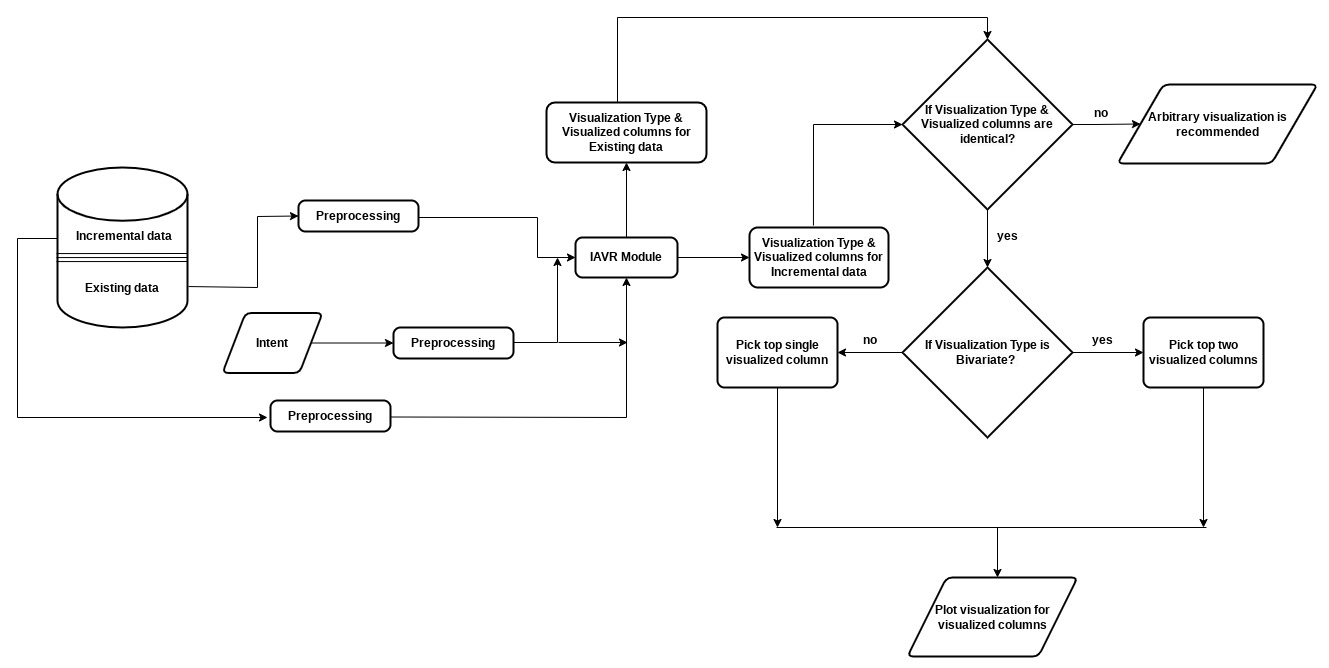
\includegraphics[width=\textwidth]{IVRIimages/flow (2).jpg}
\caption{Workflow of IVR} \label{fig1}
\end{figure}

\section{Workflow Description}

\subsection{Preprocessing:} The benchmark datasets are to be preprocessed where the missing values are replaced by median of the remaining values when the values are numeric, in other case when the data value is a string, it will be replaced with the repeated string. In addition the null values and the duplicate instances in the dataset are also removed. The preprocessed dataset is converted into the JSON format for further processing.
\subsection{Intent:} User requests are formally placed in simple sentences to visualize the data which is termed as Intent. For example Region wise insurance analysis is used as intent to obtain analysis region wise for Prediction of Insurance Charges dataset. Maruto et.al., \cite{maruta2021intent} have taken the intent as title of each visualization in a specific dataset which was crawled from Tableau public web. In our approach we analyzed the dataset and obtained the suitable intents for different datasets.
\subsection{Preprocessing Intent:} The intent is also preprocessed by removing the stop words. The words in the intent are also mapped with synonyms which could give more accurate results. The preprocessed intent is added to the dataset which is JSON format.
\subsection{Incremental dataset:} There could be two possible increments for the dataset. The increments could be instances added to the existing data which we termed as horizontal increments and adding dimensions to the existing data which we termed as vertical increments. Here we considered all possible horizontal increments and vertical increments 10\% , 20\%  till 50\% of the data size and the number of dimensions respectively. Further, the preprocessing of incremental data is also done.

\subsection{IAVR Module} 

Maruta et.al.,\cite{maruta2021intent} have proposed a visualization recommendation approach where the intent and dataset are taken as input and outputs the visualization type (Bar chart, Line chart, Pie chart etc.,), visualized columns (percentage that each column in the dataset can be part of visualization). They have used BiDA \cite{seo2016bidirectional} and BERT \cite{devlin2018bert} models for predicting the visualization type and visualized columns. Visualization type is predicted by providing both the intent embedding and the column embedding in the dataset to the BiDA model. The output of the BiDA model is given to the multilayer perceptron and softmax function is used to finally predict the visualization type. For extracting the visualized columns the intent and dataset headers are given to the pretrained BERT model. The output of the BERT model is combined with statistical features of the attributes of the dataset in order to obtain the probability of each column that could be visualized.

\begin{algorithm}[!ht]
\caption{Incremental Visualization Recommendation (IVR)}\label{algo1}
\KwIn{ Dataset (D),  Intent (I)}
\KwOut{Visualization (V)}
Preprocess D \& I

\(EV \leftarrow IAVR(D,I)\)

\If{hy = 1 and vy = 0}
{
\(IV \leftarrow IAVR(hy,I)\)
}   
\ElseIf{vy = 1 and hy = 0}
{
    \(IV \leftarrow IAVR(vy,I)\)
}
\ElseIf{vy = 1 and hy = 1}
{
    \(IV \leftarrow IAVR(hy+vy,I)\)
}
\If{EV = IV}
{
    \If{VT = 1}
    {
        \(VC \leftarrow (VC0,VC1)\)
    }
    \Else
    {    
    \(VC \leftarrow (VC0)\)
    }
}
    \(V \leftarrow plot(VT, VC)\)
    
\KwRet{V}
\end{algorithm}
\section{Algorithm Description}
The dataset and intent are taken as input. Preprocessing of the dataset and intent is done which was discussed earlier in section 3.1. Incremental data is added to the dataset horizontally (hy) and vertically (vy). hy and vy can take the value either 0 or 1 where 1 indicates increments and 0 indicates no increments. IAVR is an Intent Aware Visualization Recommendation algorithm \cite{maruta2021intent} which will give visualization (visualization type and visualized columns)  as output. IAVR is applied for existing data (D) and Intent (I) which will give a visualization recommendation and it is  termed as Existing Visualization (EV). When the data is evolving in a data stream, then IAVR \cite{maruta2021intent} is applied to the chunks of incremental data without considering the data from scratch. Ultimately, we will get a visualization recommendation exclusively for incremental data and termed as Incremental Visualization (IV). Now EV and IV recommendations are compared if both are same then visualization type (VT) is checked. VT can take the value either 0 or 1 where 1 indicates bivariate and 0 indicates univariate. If the visualization type is bivariate the top two visualized columns (VC) are chosen (VC0 \& VC1) otherwise the top visualized column is chosen (VC0). Finally visualization is plotted for the visualized columns (VC) based on visualization type (VT).




\section{Comparison between traditional and proposed approach}

\begin{table}[H]
\caption{Comparison of our proposed approach with traditional approach}\label{tab1}
\scalebox{0.56}
{
\begin{tabular}{|c|c|}
\hline
\textbf{Traditional Maruto et.al., (2021) \cite{maruta2021intent}} &  \textbf{Proposed Approach IVR}\\
\hline
Can’t handle incremental data & Handles incremental data\\
\hline
Used synthetic dataset &  Used benchmark datasets \\
\hline
Can’t handle volume and velocity in the context of data of big data & Handles volume and velocity in the context of data of big data\\
\hline
Time consuming & Less time consuming\\
\hline
\end{tabular}
}
\end{table}







\section{Discussions and Experimental results}
Experiments performed for three standard benchmark datasets of the Kaggle database i.e Prediction of Insurance Charges, AQI - Air Quality Index, California House Price. All of these datasets have different data sizes and dimensions.
We generated intents from each dataset to perform experiments and the details are provided. Later, the dataset is divided into two parts in the ratio of (90:10, 80:20, 70:30, 60:40, 50:50). First part is considered as existing data and the remaining part is considered as incremental data (it can be horizontal and vertical increments).
A pre-trained GloVe model \cite{pennington2014glove} is used for word embedding. This model was trained using the Wikipedia 2014 dump and Gigaword 5 corpus. For predicting the visualization type BiDA model is used with six layers in the multilayer perceptron \cite{maruta2021intent}. For identifying visualized columns a pre-trained BERT model is used with two layers in the multilayer perceptron \cite{maruta2021intent}. 
\subsection{Experimental Results} 
The IAVR \cite{maruta2021intent} algorithm is applied to the first part treating as existing data and obtaining the desired results. Then same algorithm is applied to the second part treating as incremental data. Comparing the visualization results (VT and VC) and recommend the visualization for the entire data (existing and incremental data). Hence, IAVR \cite{maruta2021intent} is applied for every timestamp for incremental data and recommends visualization for the entire data (existing and incremental data). 
Table 2 shows the results obtained with our proposed approach.


\begin{table}[ht]
\caption{Experimentation of our proposed approach with benchmark datasets for horizontal and vertical increments}\label{tab2}
\scalebox{0.8}{\renewcommand{\arraystretch}{2.5}
\begin{tabular}{|p{3cm}|p{3cm}|p{3cm}|p{3cm}|p{3cm}|}
\hline
\textbf{Dataset} & \textbf{Intent} & \textbf{Incremental data (Horizontal and Vertical)} & \textbf{Visualization recommendation for existing data}  & \textbf{Visualization recommendation for incremental data}       \\ \hline
\multirow{2}{*}{\parbox{3cm}{Prediction of Insurance Charges Size: 1337 X 5}} & Region wise insurance analysis & \multirow{2}{*}{\parbox{3cm}{10\%, 20\%, 30\%, 40\% and 50\% of data size and number of dimensions respectively.}} & Pie Chart for region column & Pie Chart for region column  \\
 \cline{2-2} \cline{4-5}  
 & Impact of insurance charges on having children &  & Bar Chart between having children and insurance charges & Bar Chart between having children and insurance charges
 
 \\
 \hline
\multirow{2}{*}{\parbox{3cm}{AQI - Air Quality Index\\ Size:\\ 10127 X 4}} & Air Quality Index value according to country & \multirow{2}{*}{\parbox{3cm}{10\%, 20\%, 30\%, 40\% and 50\% of data size and number of dimensions respectively.}} & Line Chart between AQI value and country & Line Chart between AQI value and country  \\
\cline{2-2} \cline{4-5}
 & Examination of population close to ocean & & Bar Chart between ocean proximity and population & Bar Chart between ocean proximity and population \tabularnewline
 \hline
\multirow{2}{*}{\parbox{3cm}{California House Price\\ Size:\\ 20640 X 10}} & House value effect on  number of bedrooms & \multirow{2}{*}{\parbox{3cm}{10\%, 20\%, 30\%, 40\% and 50\% of data size and number of dimensions respectively.}} & Bar Chart between median house value and total bedrooms & Bar Chart between median house value and total bedrooms \\
\cline{2-2} \cline{4-5}      
 & Examination of population close to ocean  &  & Bar Chart between ocean proximity and population & Bar Chart between ocean proximity and population\tabularnewline
 \hline
\end{tabular}}
\end{table}



The above tabulated results show that the visualization recommendation for the existing data and incremental data (horizontal and vertical) are the same. Hence that particular visualization is recommended for the entire data (existing and incremental data).
\subsection{Analysis of the results }
Experimentation done on the benchmark Air Quality Dataset by considering the range from 2000 instances till 10000 instances in an incremental fashion and we have observed that our proposed (incremental) approach has taken considerably less time than the traditional approach  which is depicted in Fig.~\ref{fig3}.

\begin{figure}[ht]
\centering
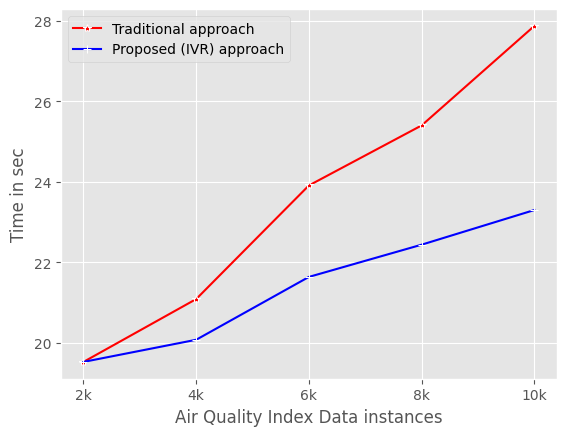
\includegraphics[height=5cm,width=9cm]{IVRIimages/time (2).png}
\caption{Workflow of IVR} \label{fig3}
\end{figure}


In our experimentation we have considered two cases to analyze the results. When the instances are added to the existing data those are considered as horizontal increments which we categorized as Case 1 and dimensions are added to the existing data those are considered as vertical increments which we categorized as Case 2.\\
\textbf{Case 1:}\\
When horizontal increments are added to the data, the visualization recommendation by our approach is the same for the existing and incremental data.\\
\textbf{Case 2:}\\
There are again two phases with vertical increments.
\begin{itemize}
    \item The added dimension names are not part of the intent 
    \item The added dimension names are part of the intent
\end{itemize}

When the added dimension names are not part of the intent, the visualization recommendation by our approach is the same for the existing and incremental data. When the dimension names are part of the intent, we observed that in some cases the visualization recommendation for existing and incremental data is different then arbitrary visualization recommendation is suggested. The details of this work are in progress but beyond the scope of this paper.
\chapter{\Large \texorpdfstring{$HM\_QCv$}{HM\_QCv}: A Computationally Efficient Hybrid Model for Enhancing Quality Clusters in Visualization}



Traditional techniques \cite{tsne} \cite{umap_reference} \cite{sun2023laplacian} exist for visualizing high-dimensional data. Still, they face limitations by covering all characteristics, such as (i) minimizing computational costs, (ii) providing high-quality cluster visualizations, and (iii) preserving both local and global structures. Local structures refer to the relationships between nearby data points \cite{tsne}, whereas global structures encompass the overall distribution of the data \cite{umap_reference} \cite{tenenbaum2000global}.

Sun et al. \cite{sun2023laplacian} developed an approach that uses the t-SNE \cite{tsne} methodology to preserve the local and global structure and incorporates a symmetric Laplacian matrix, the regularization technique for cluster quality when visualizing the data. However, this approach, while improving the representation of clusters, also increases the computational complexity due to t-SNE \cite{tsne}.

The existing methodology LAPtSNE \cite{sun2023laplacian}, relies on the t-SNE \cite{tsne} method to compute the distance between the data objects, which is computationally intensive.  To address this limitation, we adopted UMAP \cite{umap_reference} in our proposed approach.  Before adopting UMAP \cite{umap_reference}, we conducted experiments on three benchmark datasets to evaluate both the t-SNE \cite{tsne} and UMAP \cite{umap_reference} approaches, measuring their processing times. The results clearly demonstrate that UMAP \cite{umap_reference} is more computationally efficient than t-SNE \cite{tsne}. Hence, our approach, $HM\_QCv$, is more computationally efficient than LAPtSNE \cite{sun2023laplacian} while ensuring both local and global structure by preserving high-quality cluster visualization, offering promising practical implications for the field of data visualization.


The $HM\_QCv$ approach is designed to preserve both (i) cluster information and (ii) local and global structures of high-dimensional data in visualization. Our approach leverages the strengths of UMAP \cite{umap_reference} and LAPtSNE \cite{sun2023laplacian} while integrating their partial components to develop more comprehensive solutions. This combined method may reveal insights that would be unattainable with either technique used independently. By leveraging UMAP \cite{umap_reference} and LaptSNE \cite{sun2023laplacian}, our approach ensures computational efficiency and significantly reduces processing time compared to LAPtSNE \cite{sun2023laplacian}.
\chapter{Incremental Visualization Recommendation based on Feature Selection}

Visualization Recommendations play a crucial role in facilitating data-driven decision-making processes. These recommendations help users to select the most appropriate visualizations for a dataset. This ensures that information is presented in a clear, accurate, and precise manner, promoting better understanding and insight extraction. Effective visualization recommendations also consider the user's interest and intended applications. In an era where data is abundant, data visualization recommendations are helpful to achieve accurate results and require a better understanding of any dataset extensively to make decisions. 

According to Maruta et al. \cite{maruta2021intent}, Visualization Recommendations for the dataset are categorized into Machine Learning, Rule-based and Knowledge Graph approaches \cite{li2021kg4vis}. These approaches often struggle with scalability and complexity, particularly when handling high-dimensional data or large-scale knowledge graphs. Rule-based approaches \cite{mackinlay1986automating, mackinlay2007show, roth1994interactive, wongsuphasawat2017voyager, stolte2002polaris} have a limitation as they require expert intervention. Machine Learning approaches \cite{qian2020ml, hu2019vizml, dibia2019data2vis, luo2018deepeye, moritz2018formalizing} require dataset visualization pairs, and obtaining those pairs will be very difficult. Knowledge Graph approaches require a huge amount of data to construct the knowledge graph, which is a major hindrance. 

To address the above-discussed limitations, Maruta et al. \cite{maruta2021intent} proposed an alternate approach based on users requirements termed \textbf{Intent}. Intent is used for the dataset to filter and choose the columns from the dataset to visualize the data. This approach of using user intent to recommend visualizations can be problematic if the users intent is not specified accurately or if the dataset includes several features that correspond to the same intent, resulting in ambiguity.
   
Therefore, selecting the visualized columns to recommend the visualization for the dataset without using the users intent was quite challenging. To address these limitations, we plan to propose a Feature Selection based approach to select the columns to be visualized from the dataset, which were used to recommend the visualization without using the Intent.

Visualization Recommendation for the incremental data with respect to Volume and Velocity in terms of Big Data generated over time is critical to handle. One of our works Kuruva et al. \cite{kuruva2023visualization}, handles the incremental data exclusively and recommends the appropriate visualization. This approach adopts the Intent \cite{maruta2021intent} for existing and incremental data, and the visualization for the entire dataset is further recommended. According to \cite{kuruva2023visualization}, Intent based approach \cite{maruta2021intent} fails when the Intent is not specified by the user, which sometimes results in an incorrect recommendation. There is a demand for an alternative approach that doesn't use any Intent but still recommends accurate visualization for the Incremental data. To address these limitations, we plan to propose an Incremental Visualization Recommendation using Feature Selection \textbf{(IVR\_FS)} where the new features are considered Incremental data. 



\chapter{Conclusions and Future Work}

\section{Conclusions}

Visualization plays a key role in extracting meaningful insights from the dataset. Some visualization recommendation approaches rely on existing knowledge to obtain the recommendations, but they are often required to be processed from scratch to recommend the visualization for incremental data. Therefore, We proposed the IVR\_I approach, which is unique and recommends the visualization for the incremental added over time based on the user's specific requirements provided as Intent. There are existing NLDR approaches for visualizing the high-dimensional data, but they fail to capture the cluster information. To address this, We proposed HM\_QCv that preserves the local structure, global structure, and cluster information. 

\section{Future Work}

With our proposed IVR, we are introducing an Incremental Visualization Recommendation that is not reliant on the user-specified Intent. Instead, it is based on Feature Selection, a crucial component that provides a potential solution when user Intent is not provided alongside the dataset.

% Uncomment the following lines if you have appendices and references
%\input{./appendix.tex}
%\input{./references.bib}
%\mbox{}
%\nocite{*}
%\bibliographystyle{ieeetr}
%\printbibliography

\newpage
\bibliography{references}
\bibliographystyle{ieeetr}

\end{document}
